\section{Una panoramica}
In questo ultimo capitolo passiamo in rassegna i framework esistenti per l'implementazione di reti neurali. Grazie a loro  lo sviluppo di modelli e il processo di acquisizione dati per l'allenamento dei dati diventa molto più facile e accessibile rispetto ad un tempo. 
\begin{figure}[hbtb]
\centering
\subfloat[][\emph{Keras}]
{
\includegraphics[scale=0.5]{media_tesi/keras_logo.png}} \hspace{1.5cm}\vspace{1cm}
\subfloat[][\emph{TensorFlow}]
{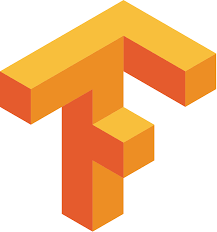
\includegraphics[scale=0.5]{media_tesi/ts_logo.png}} \hspace{1.5cm}
\vspace{1cm}
\subfloat[][\emph{PyTorch}]
{
\includegraphics[scale=0.6]{media_tesi/pytorch_logo.png}} \hspace{1.5cm}
\subfloat[][\emph{Caffe 2}]
{
\includegraphics[scale=0.6]{media_tesi/caffe2_logo.png}} \hspace{1.5cm}
\subfloat[][\emph{theano}]
{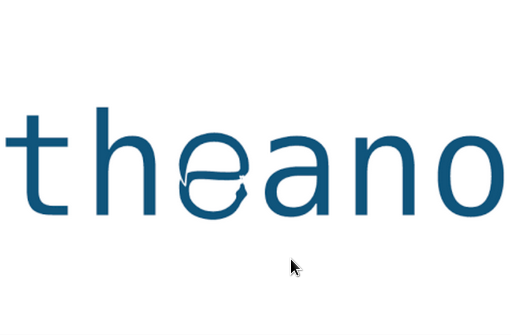
\includegraphics[scale=0.3]{media_tesi/theano_logo.png}} \hspace{1.5cm}
\subfloat[][\emph{mxnet}]
{
\includegraphics[scale=0.4]{media_tesi/mx_logo.png}}\\ 

\vspace{1cm}
\caption{I loghi dei principali framework per le reti neurali}
\label{fig:subfig}
\end{figure}

\section{TensorFlow}
TensorFlow  fu creato dal team Brain Google come successore di un precedente sistema per il machine learning conosciuto come \textit{DistBelief} con l'intento di ristrutturare il codice rendendola una libreria più robusta \cite{wiki:tf}. Venne distribuita come progetto open-source nel 2015 e si presenta come un framework di basso livello \cite{oreilly:pytorch_intro} per linguaggi come Python, Javascript, Swift e Java per Android  e le librerie a cui fa a sua volta ricorso per l'implementazione delle parti più critiche sono scritte in C++. TensorFlow, vista una sua certa difficoltà d'uso e apprendimento, offre compatibilità con le API d'alto livello di \textit{Keras}; esse consentono grazie alla loro modularità e facilità di utilizzo di eseguire velocemente la prototipizzazione di modelli e la sperimentazione delle reti neurali su piattaforme diverse e renderle velocemente funzionanti per il testing \cite{keras}.

TensorFlow rappresenta le computazioni come dei grafi i quali sono composti da due tipi di oggetti: le operazioni, ovvero i nodi del grafo e i tensori, dal cui utilizzo prende il nome, che sarebbero gli archi del grafo.
I tensori sono matrici multidimensionali su cui vengono fatti i calcoli e che contengono i parametri della rete.

TensorFlow gira sia su CPU che GPU, grazie alle librerie di programmazione per schede grafiche \textit{CUDA} e \textit{OpenCL}. Per la sua applicazione specifica è stato progettato da Google un processore dedicato chiamato \emph{Tensor Processing Unit} \textit{TPU}. L'interesse verso un processore dedicato non tanto all'allenamento della rete quanto al suo utlizzo rappresenta un vantaggio per l'applicazione dell'intelligenza artificiale in quegli ambiti dove si predilige una velocità di esecuzione; un esempio può essere un chip dedicato in un dispositivo cellulare, che rende più efficiente determinati task, come il riconoscimento vocale o facciale per quelle applicazioni che ne fanno uso. Google stessa dichiarò che il suo utilizzo nei datacenter aveva ottimizzato le performance di un ordine di grandezza, riducendo il dispendio energetico derivato dal loro utilizzo \cite{gao2014machine}. 

TensorFlow presenta anche diverse problematiche come la sua difficoltà di utilizzo: ecco perchè Keras si appoggia al di sopra di esso, come dicevamo in precedenza.

\section{PyTorch}
Questo framework uscì nel 2016 e si ispirò fortemente ad altri framework come \textit{Chainer} e \textit{Torch}. Pytorch si indirizzava le problematiche di adozione che colpivano Torch e a questo proposito si decise di utilizzare come linguaggio d'utilizzo per gli utenti Python. Il suo approccio è un pò diverso da quello di Tensorflow in quanto l'esecuzione delle operazioni nel grafico computazionale avvengono immediatamente mentre in TensorFlow il grafico è compilato ed eseguito in un colpo solo e questo rende possibile un debugging più dinamico. Infatti costituisce un rallentamento l'immaginare un modello e dover fare i conti con gli errori della sua progettazione soltanto a termine di questa, è molto più produttivo correggere gli errori via via che si presentano. 

Pytorch è sviluppato e mantenuto dal team per l'intelligenza artificial di Facebook (\textit{FAIR}) e la sua adozione presso gli utenti è stata molto più ampia rispetto a quella del suo predecessore. Viene apprezzato per la familiarità che ricercatori e data scientist avevano già nei confronti di Python mentre a livello commerciale gli vengono preferite alternative in quanto i modelli di PyTorch non sono facilmente portabili su mobile \cite{oreilly:pytorch_intro}.

Negli stessi laboratori di Facebook la strategia è quella di utilizzare PyTorch nella ricerca e Caffe2 per la produzione.

PyTorch offre supporto ai dispositivi CUDA con Python e un frontend C++ \cite{pytorch:docs}.

\section{Caffe2}
Arriviamo a quest'altro progetto per le reti neurali sviluppato da Facebook, il più giovane fra quelli che presentiamo. \textit{Caffe2} trae origine da \textit{Caffe}, il quale offriva un ottimo supporto alla produzione di applicazioni che lavorassero bene su larga scala, grazie al suo codice sorgente scritto in C++ \cite{caffe_intro}. Rispetto al predecessore si evidenzia la modularità e il forte orientamento al mondo mobile, con applicazioni nella visione artificiale e il riconoscimento del linguaggio \cite{wiki:caffe2}. Facebook annunciò la pubblicazione open-source di Caffe2 il 18 aprile 2017 con il proposito di rilasciare un framework leggero che fosse portabile su più piattaforme ma che mantenesse la capacità di scalare bene e performare\cite{caffe_announcement}.

Caffe2 è principalmente utilizzato in Python ma può anche essere importato in progetti C++ anche se la disponibilità online di documentazioni relative a questo connubio sono piuttosto difficili da trovare \cite{caffe_c++} e si può anche utilizzare le GPU grazie al supporto CUDA.

\section{Mxnet}
Mxnet è un framework sviluppato dalla \textit{Apache Software Foundation} con l'intento di renderlo molto efficiente, produttivo e flessibile. Può infatti essere usato da diversi linguaggi come Python, C++, R, Julia e Scala per citarne solo alcuni, il che lo rende molto appetibile poichè non richiede di imparare un nuovo linguaggio per il suo utilizzo. Il suo backend è scritto in \emph{C++} e \emph{CUDA} e presenta un'ottima capacità a scalare linearmente e a scaricare il suo workload su molteplici GPU \cite{maruti:mxnet}. Inoltre il suo modello di programmazione (programming model) è molto vicino a quello di Keras, senza gli svantaggi delle performance in quanto è tutto nativo \cite{quora:mxnet}.

La bontà del progetto della Apache è testimoniata anche dalla sua adozione da parte di Amazon Web Services (AWS) come principale framework per il deep-learning che ha inoltre deciso di finanziarne lo sviluppo suo e dell'ecosistema di applicazioni che lo supportano \cite{aws-mxnet}. 
\section{Theano}
Un altro framework che merita una menzione è Theano, libreria per Python che consente di definire, ottimizzare e valutare espressioni matematiche che coinvolgono strutture di array multidimensione. 
Theano è stato sviluppato dall'Università di Montreal in Canada e dal 2007 viene utilizzato per far funzionare grandi carichi di lavoro su larga scala. La sua implementazione sfrutta pesantemente una parte del codice di \emph{Numpy}, un'altra libreria per Python ed è in grado di supportare le computazioni anche su GPU \cite{2016arXiv160502688short}.

Il 28 settembre 2018 hanno inoltre annunciato l'interruzione del suo sviluppo a causa della concorrenza del mondo industriale \cite{lamblin}. Questo significa che Theano non verrà usato in nuove applicazioni, sebbene possa rimanere presente in applicazioni legacy.
